\documentclass[12pt,a4paper]{article}
\usepackage[utf8]{inputenc}
\usepackage[T1]{fontenc}
\usepackage{geometry}
\usepackage{tikz}
\usetikzlibrary{er,positioning,shapes.geometric,arrows.meta}
\usepackage{hyperref}
\usepackage{fancyhdr}

\geometry{margin=2.5cm}
\pagestyle{fancy}
\fancyhf{}
\fancyhead[L]{GovEase - Entity-Relationship Diagram}
\fancyfoot[C]{\thepage}

\title{\textbf{GovEase Government Services Management System\\Entity-Relationship Diagram}}
\author{BitByBit Development Team}
\date{\today}

\begin{document}

\maketitle

\section{Entity-Relationship Diagram}

\begin{figure}[h!]
\centering
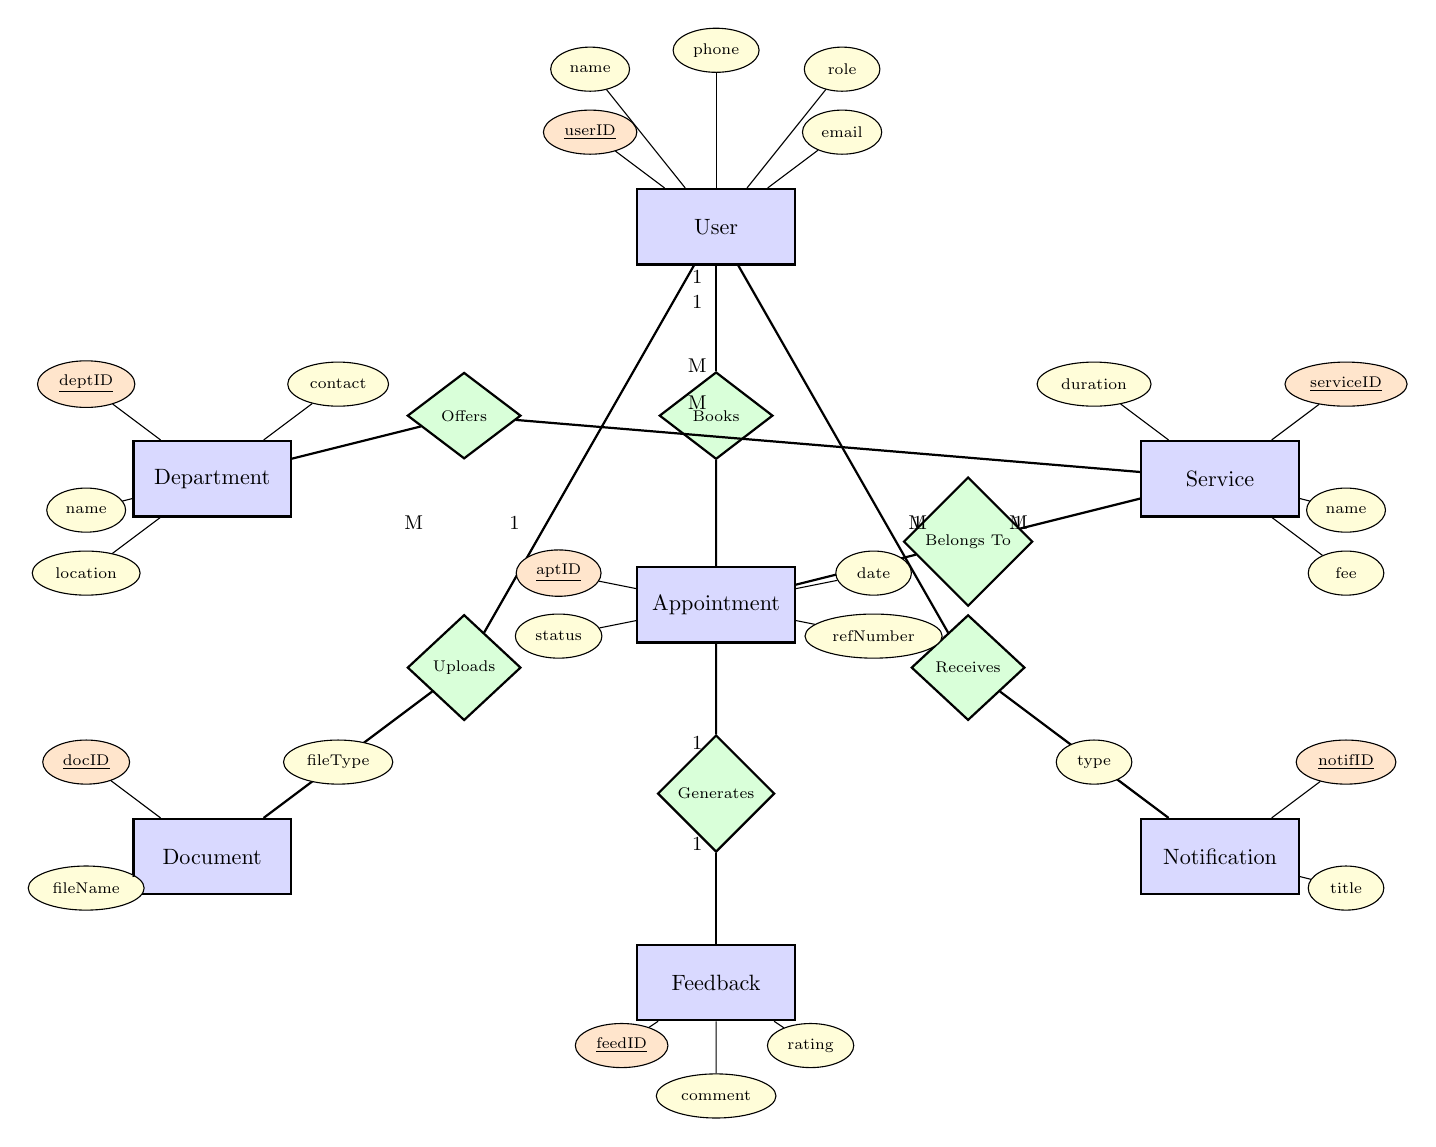
\begin{tikzpicture}[scale=0.8, transform shape]

% Define styles
\tikzstyle{entity} = [rectangle, draw=black, thick, text centered, minimum height=1.2cm, minimum width=2.5cm, fill=blue!15]
\tikzstyle{attribute} = [ellipse, draw=black, text centered, minimum height=0.7cm, minimum width=1.2cm, fill=yellow!15, font=\scriptsize]
\tikzstyle{relationship} = [diamond, draw=black, thick, text centered, minimum height=0.8cm, minimum width=1.8cm, fill=green!15, font=\scriptsize]
\tikzstyle{primarykey} = [attribute, fill=orange!20]

% Main entities positioned in a clear layout
\node [entity] (user) at (0,6) {User};
\node [entity] (dept) at (-8,2) {Department};
\node [entity] (service) at (8,2) {Service};
\node [entity] (appointment) at (0,0) {Appointment};
\node [entity] (document) at (-8,-4) {Document};
\node [entity] (notification) at (8,-4) {Notification};
\node [entity] (feedback) at (0,-6) {Feedback};

% Relationships
\node [relationship] (books) at (0,3) {Books};
\node [relationship] (offers) at (-4,3) {Offers};
\node [relationship] (belongsto) at (4,1) {Belongs To};
\node [relationship] (uploads) at (-4,-1) {Uploads};
\node [relationship] (receives) at (4,-1) {Receives};
\node [relationship] (generates) at (0,-3) {Generates};

% Primary connections
\draw [thick] (user) -- (books);
\draw [thick] (books) -- (appointment);
\draw [thick] (dept) -- (offers);
\draw [thick] (offers) -- (service);
\draw [thick] (service) -- (belongsto);
\draw [thick] (belongsto) -- (appointment);
\draw [thick] (user) -- (uploads);
\draw [thick] (uploads) -- (document);
\draw [thick] (user) -- (receives);
\draw [thick] (receives) -- (notification);
\draw [thick] (appointment) -- (generates);
\draw [thick] (generates) -- (feedback);

% Cardinality labels
\node [font=\small] at (-0.3,5.2) {1};
\node [font=\small] at (-0.3,3.8) {M};
\node [font=\small] at (-0.3,4.8) {1};
\node [font=\small] at (-0.3,3.2) {M};
\node [font=\small] at (3.2,1.3) {M};
\node [font=\small] at (4.8,1.3) {1};
\node [font=\small] at (-3.2,1.3) {1};
\node [font=\small] at (-4.8,1.3) {M};
\node [font=\small] at (3.2,1.3) {1};
\node [font=\small] at (4.8,1.3) {M};
\node [font=\small] at (-0.3,-2.2) {1};
\node [font=\small] at (-0.3,-3.8) {1};

% Key attributes for User
\node [primarykey] (user_id) at (-2,7.5) {\underline{userID}};
\node [attribute] (user_email) at (2,7.5) {email};
\node [attribute] (user_name) at (-2,8.5) {name};
\node [attribute] (user_role) at (2,8.5) {role};
\node [attribute] (user_phone) at (0,8.8) {phone};

% Key attributes for Department
\node [primarykey] (dept_id) at (-10,3.5) {\underline{deptID}};
\node [attribute] (dept_name) at (-10,1.5) {name};
\node [attribute] (dept_location) at (-10,0.5) {location};
\node [attribute] (dept_contact) at (-6,3.5) {contact};

% Key attributes for Service
\node [primarykey] (service_id) at (10,3.5) {\underline{serviceID}};
\node [attribute] (service_name) at (10,1.5) {name};
\node [attribute] (service_fee) at (10,0.5) {fee};
\node [attribute] (service_duration) at (6,3.5) {duration};

% Key attributes for Appointment
\node [primarykey] (apt_id) at (-2.5,0.5) {\underline{aptID}};
\node [attribute] (apt_date) at (2.5,0.5) {date};
\node [attribute] (apt_status) at (-2.5,-0.5) {status};
\node [attribute] (apt_ref) at (2.5,-0.5) {refNumber};

% Key attributes for Document
\node [primarykey] (doc_id) at (-10,-2.5) {\underline{docID}};
\node [attribute] (doc_name) at (-10,-4.5) {fileName};
\node [attribute] (doc_type) at (-6,-2.5) {fileType};

% Key attributes for Notification
\node [primarykey] (notif_id) at (10,-2.5) {\underline{notifID}};
\node [attribute] (notif_title) at (10,-4.5) {title};
\node [attribute] (notif_type) at (6,-2.5) {type};

% Key attributes for Feedback
\node [primarykey] (feed_id) at (-1.5,-7) {\underline{feedID}};
\node [attribute] (feed_rating) at (1.5,-7) {rating};
\node [attribute] (feed_comment) at (0,-7.8) {comment};

% Connect attributes to entities
\draw (user) -- (user_id);
\draw (user) -- (user_email);
\draw (user) -- (user_name);
\draw (user) -- (user_role);
\draw (user) -- (user_phone);

\draw (dept) -- (dept_id);
\draw (dept) -- (dept_name);
\draw (dept) -- (dept_location);
\draw (dept) -- (dept_contact);

\draw (service) -- (service_id);
\draw (service) -- (service_name);
\draw (service) -- (service_fee);
\draw (service) -- (service_duration);

\draw (appointment) -- (apt_id);
\draw (appointment) -- (apt_date);
\draw (appointment) -- (apt_status);
\draw (appointment) -- (apt_ref);

\draw (document) -- (doc_id);
\draw (document) -- (doc_name);
\draw (document) -- (doc_type);

\draw (notification) -- (notif_id);
\draw (notification) -- (notif_title);
\draw (notification) -- (notif_type);

\draw (feedback) -- (feed_id);
\draw (feedback) -- (feed_rating);
\draw (feedback) -- (feed_comment);

\end{tikzpicture}
\caption{Entity-Relationship Diagram for GovEase Database}
\label{fig:er_diagram}
\end{figure}

\section{Entity Descriptions}

\begin{itemize}
\item \textbf{User}: Represents citizens, officers, and administrators using the system
\item \textbf{Department}: Government departments offering services
\item \textbf{Service}: Specific services offered by departments
\item \textbf{Appointment}: Scheduled appointments for services
\item \textbf{Document}: Files uploaded by users for appointments
\item \textbf{Notification}: System notifications sent to users
\item \textbf{Feedback}: User feedback on completed appointments
\end{itemize}

\section{Relationships}

\begin{itemize}
\item \textbf{Users ↔ Appointments}: One-to-Many (A user can have multiple appointments)
\item \textbf{Departments ↔ Services}: One-to-Many (A department offers multiple services)
\item \textbf{Services ↔ Appointments}: One-to-Many (A service can have multiple appointments)
\item \textbf{Appointments ↔ Documents}: One-to-Many (An appointment can have multiple documents)
\item \textbf{Users ↔ Notifications}: One-to-Many (A user can receive multiple notifications)
\item \textbf{Appointments ↔ Feedback}: One-to-One (Each appointment can have one feedback)
\end{itemize}

\end{document}